\begin{solution}

\begin{enumerate}
\item {[8 points]} We compute
  \begin{eqnarray*}
     {\d u\over \d t} &=& -\frac{\kappa \theta^2}{\rho c} e^{-\kappa \theta^2 t/(\rho c)} \sin(\theta x) \\[0.5em]
     {\d u\over \d x} &=& \theta e^{-\kappa \theta^2 t/(\rho c)} \cos(\theta x) \\[0.5em]
     {\d^2 u\over \d x^2} &=& -\theta^2 e^{-\kappa \theta^2 t/(\rho c)} \sin(\theta x).
  \end{eqnarray*}
Hence,
 \[  \rho c {\d u \over \d t} = -\kappa \theta^2 e^{-\kappa \theta^2 t/(\rho c)} \sin(\theta x)\]
and
 \[  \kappa {\d^2 u\over \d x^2} = -\kappa \theta^2 e^{-\kappa \theta^2 t/(\rho c)} \sin(\theta x)\]
from which it can be seen that
 \[  \rho c {\d u \over \d t} = \kappa {\d^2 u\over \d x^2}.\]

\item {[8 points]} We wish to find the values of $\theta$ that give homogeneous Dirichlet boundary conditions,
      i.e., $u(0,t) = u(\ell,t)=0$ for all $t$.
      Since $e^{-\kappa \theta^2 t/(\rho c)}$ is positive for all $t$, we can only get
      the homogeneous Dirichlet conditions when $\sin(\theta x)=0$.
      For any $\theta$, $\sin(\theta\cdot 0) = 0$, so the condition at $x=0$ is automatically
      satisfied.  To get $\sin(\theta \ell) = 0$, we need $\theta \ell$ 
      to be an integer multiple of $\pi$, that is,
           \[ \theta \ell = \pi n, \qquad n = 0, \pm 1, \pm 2, \ldots,\]
      or equivalently
           \[ \theta  = {\pi n\over \ell}, \qquad n = 0, \pm 1, \pm 2, \ldots.\]

\item {[9 points]}

      Notice that if $n=0$ we have the trivial solution $u(x,t) =0 $ for $0\le x\le\ell$ and all $t$.
       If $n=1$, we have a solution for which $u(x,t) \ge 0$ for $0\le x\le\ell$ and all $t$.
       For other values of $n$ the solution will be \emph{negative} for some $x\in[0,\ell]$.
       If our temperature is measured in Kelvin this could be a problem!
       However, this heat equation takes the same form if we shift to Celsius units,
       so we needn't be so troubled by the negative values of temperature.

Since $n=0$ is trivial, we shall take $n=1$ ($\theta = \pi/\ell$) to obtain       
                  \begin{eqnarray*}
                        u(x,t) &=& e^{-\kappa \pi^2 t/(\ell^2 \rho c)} \sin(\pi x/\ell)  \\[0.5em]
                               &=& e^{-2.37 \pi^2 t/(100\cdot 2.70\cdot 0.897)} \sin(\pi x/10).
                  \end{eqnarray*}
Solutions are shown in the attached plots.  Any of these style is acceptable. 
      The MATLAB code that generated these plots follows. 


        
      \begin{center}
           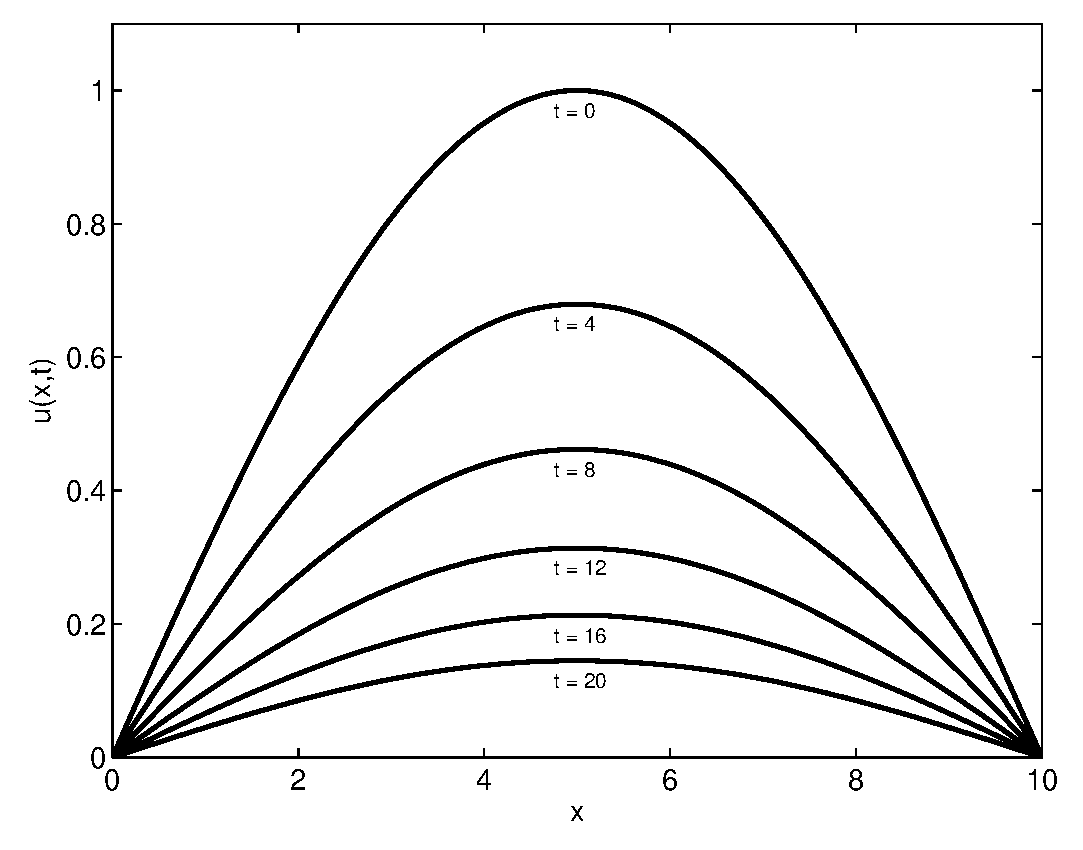
\includegraphics[scale=0.53]{checksol1}

           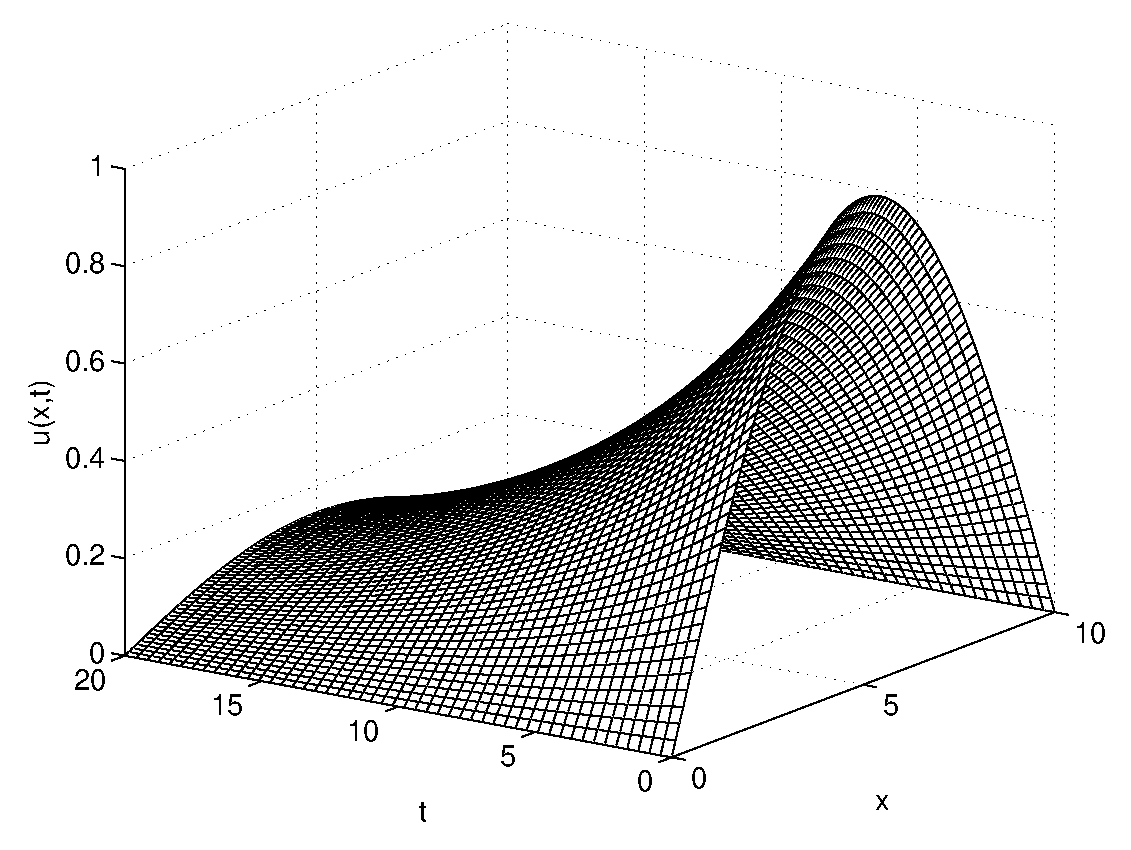
\includegraphics[scale=0.53]{checksol2}

           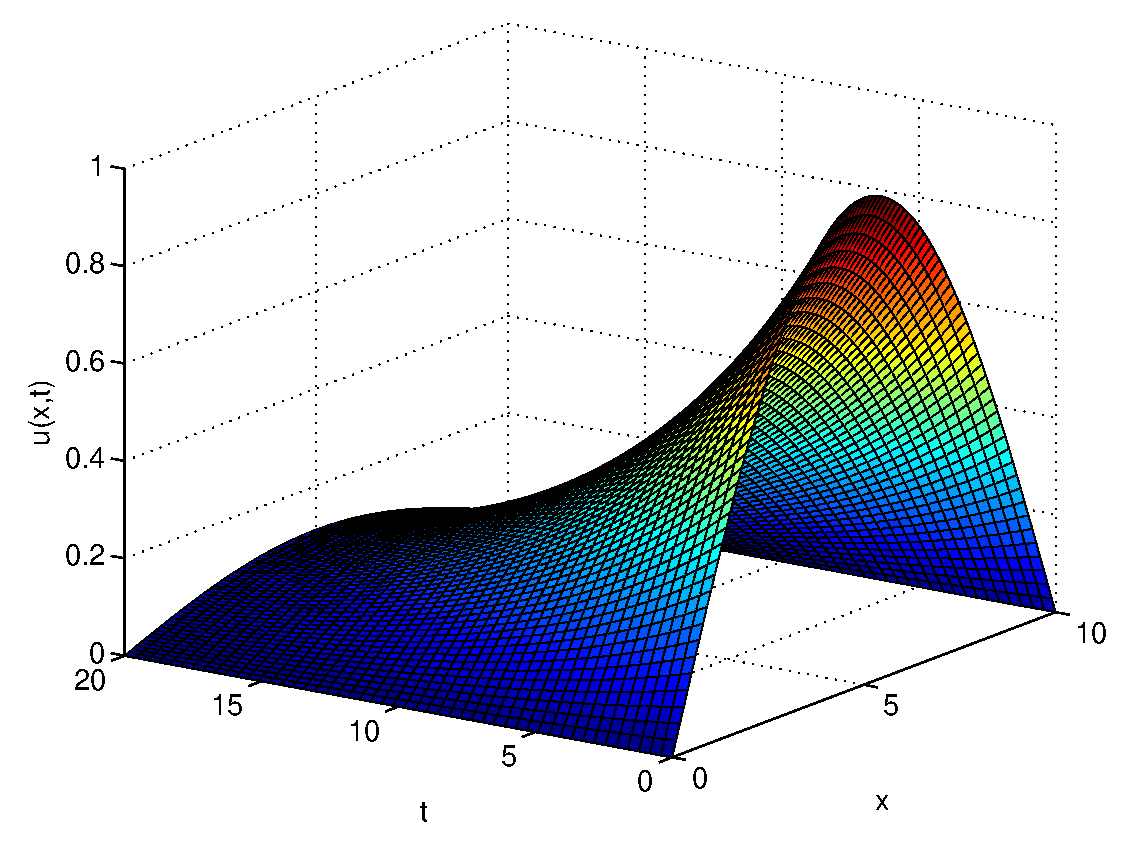
\includegraphics[scale=0.53]{checksol3}

           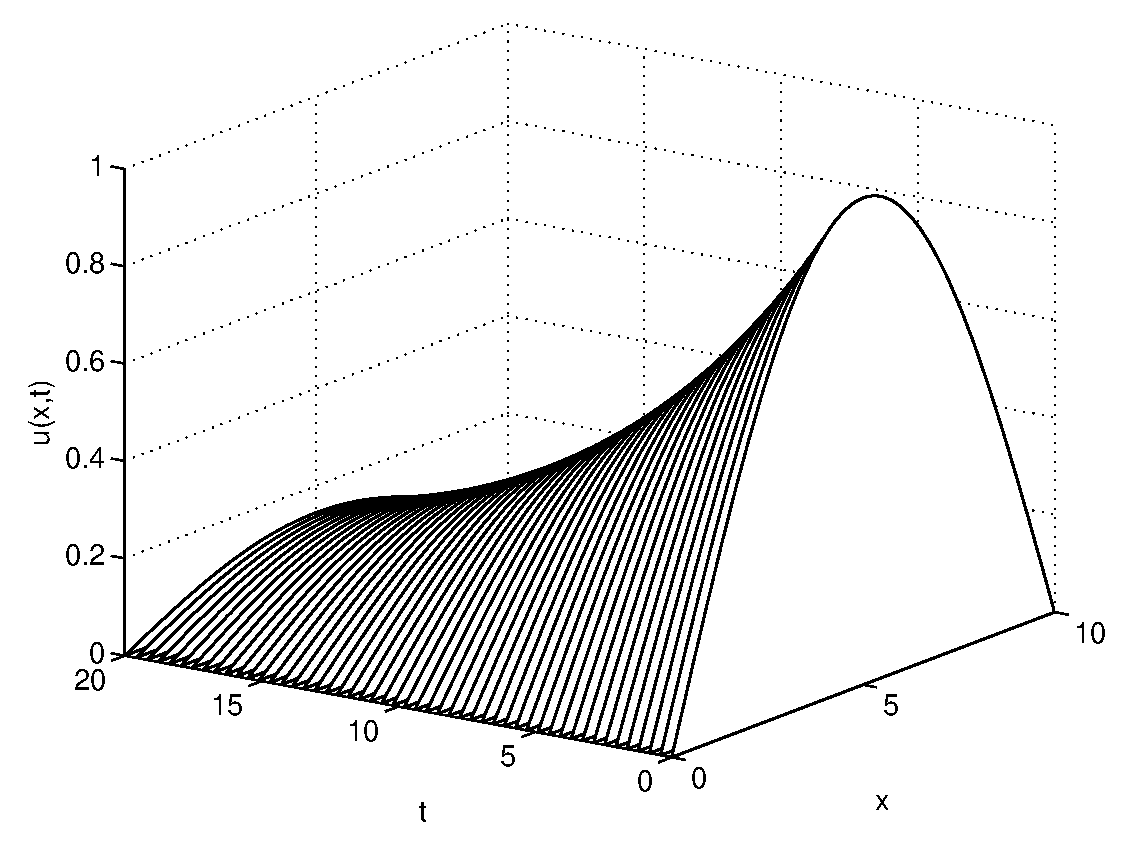
\includegraphics[scale=0.53]{checksol4}

           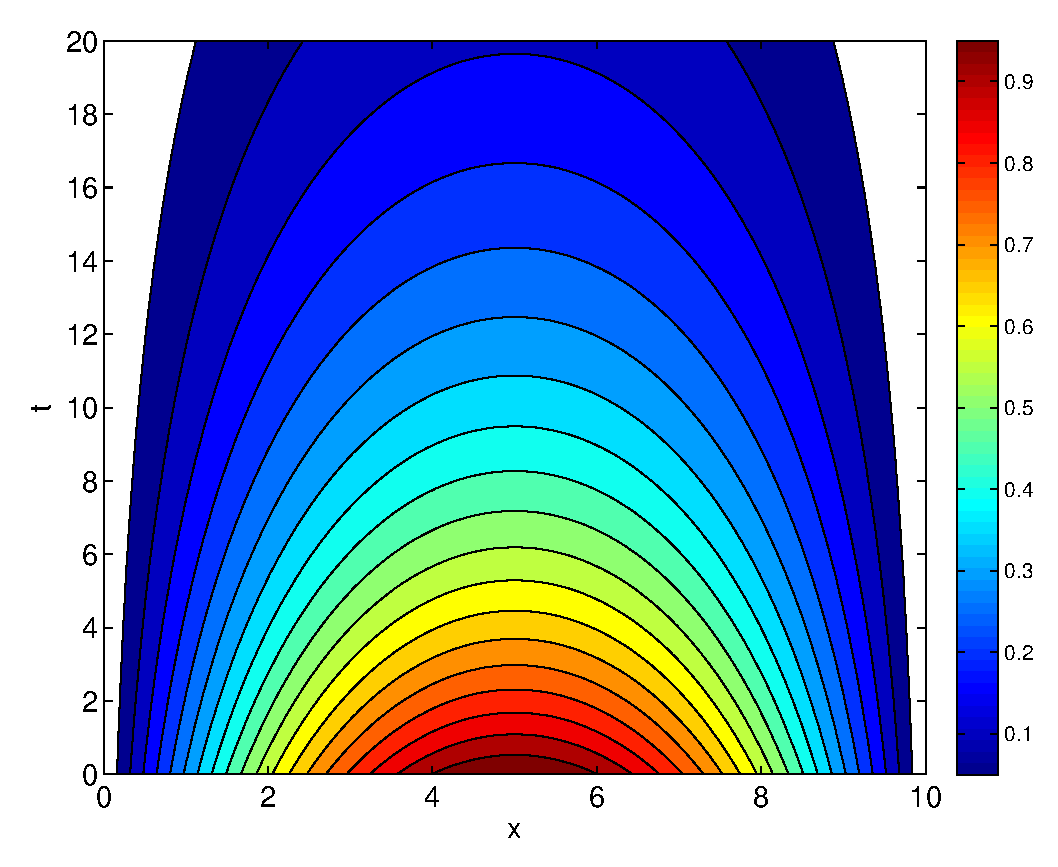
\includegraphics[scale=0.53]{checksol5}
      \end{center}

MATLAB code:

\lstinputlisting{HW7c.m}

\end{enumerate}
\end{solution}

